\documentclass{article}
\usepackage{pgfplots}
\usetikzlibrary{patterns}
\pagenumbering{gobble}
\pgfplotsset{compat=1.9}
\begin{document}
\noindent
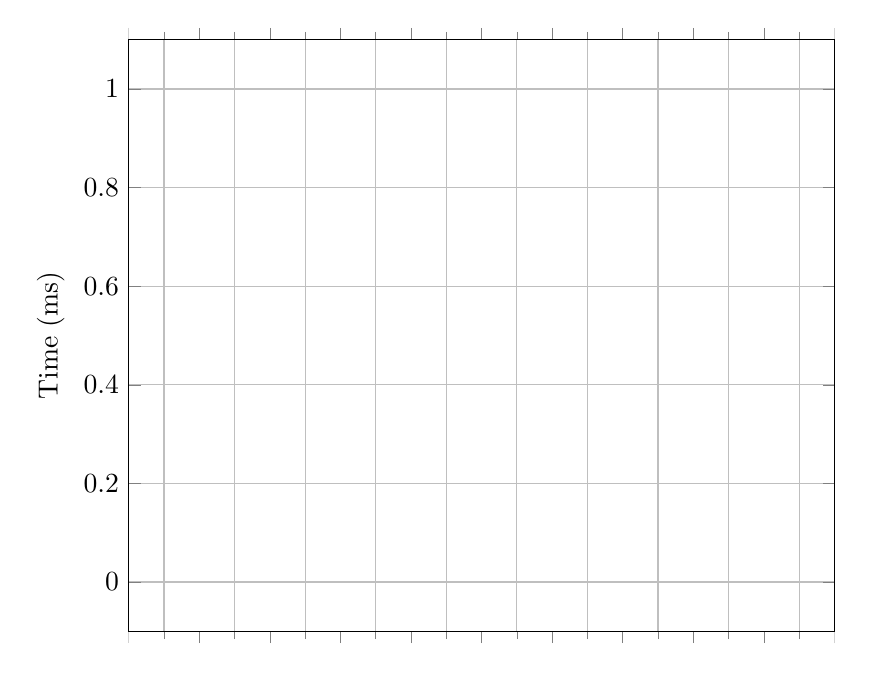
\begin{tikzpicture}
  \begin{axis}[
    ybar,
    % xlabel=Test,
    ylabel=Time (ms),
    width = 300,
    % enlargelimits=-0.05,
    /pgf/number format/1000 sep={},
    legend image post style={scale=2},
    legend columns = 2,
    legend style={at={(1.15,1.2)},
      % nodes={scale=0.5, transform shape},
      % anchor=north east,
      % legend columns=-1
      /tikz/column 2/.style={column sep=5pt,},
    },
    xtick={[[xtick]]},
    xticklabels={[[xticklabels]]},
    xticklabel style = {align=center},
    minor x tick num=1,
    xmajorgrids={false},
    xminorgrids={true},
    ymajorgrids={true},
    yminorgrids={false},
    xmin=0.5,xmax=3.5,
%    ymin=0,ymax=10,
    nodes near coords,
    point meta=explicit symbolic,
    % nodes near coords align={horizaontal},
    every node near coord/.append style={xshift=0.2cm,yshift=+0.8cm,rotate=90,color=black},
  ]
  [[content]]
    \legend{[[legend]]}
  \end{axis}
\end{tikzpicture}
\end{document}

%%% Local Variables:
%%% mode: latex
%%% TeX-master: t
%%% End: